\documentclass[11pt]{article}

\usepackage{listings}
\usepackage{fancyhdr}
\usepackage[margin=.8in]{geometry}
\usepackage{amsmath}
\usepackage{enumitem}
\usepackage{hyperref}
\usepackage{tikz}
\usetikzlibrary{arrows}

\tikzset{
    treenode/.style = {align=center, inner sep=2pt, text centered, font=\sffamily},
    node_num/.style = {treenode, circle, black, font=\sffamily\bfseries, draw=black, fill=white, text width=1.5em},
    node_highlight/.style = {treenode, circle, red, draw=red, text width=1.5em, very thick},
    node_null/.style = {treenode, rectangle, draw=white, minimum width=0.5em, minimum height=0.5em}
}

\linespread{1}
\setlength{\parindent}{0pt}
\setlength{\tabcolsep}{20pt}

% ===========================================================================
% Header / Footer
% ===========================================================================

\pagestyle{fancy}
\lhead{\scriptsize  CSC 212: Data Structures and Abstractions - Spring 2018}\chead{}\rhead{\scriptsize Weekly Problem Set \#11}
\lfoot{}\cfoot{\scriptsize \thepage~of~\pageref{r:lastpage}}\rfoot{}
\renewcommand{\headrulewidth}{0.25pt}
\renewcommand{\footrulewidth}{0.25pt}

% ===========================================================================
% ===========================================================================
\begin{document}
\thispagestyle{empty}

% ===========================================================================
\begin{center}
    {\Large\bf CSC 212: Data Structures and Abstractions}\\
    \medskip
    {\Large\bf Spring 2018}\\
    \medskip
    {\Large\bf University of Rhode Island}\\
    \bigskip
    {\Large\bf Weekly Problem Set \#11 Solutions}
\end{center}

Due Thursday 4/19 before class. Please turn in neat, and organized, answers hand-written on standard-sized paper \textbf{without any fringe}. At the top of each sheet you hand in, please write your name, and ID.
The only library you're allowed to use in your answers is \verb|iostream|.

\section{Binary Search Trees}
\begin{enumerate}
    
    \item Draw a binary search tree after the following operations steps:
    \begin{enumerate}
        
        \item Insert: [10, 5, 12, 8, 19, 6, 2, 11, 15, 9, 7]
        
        \begin{center}
            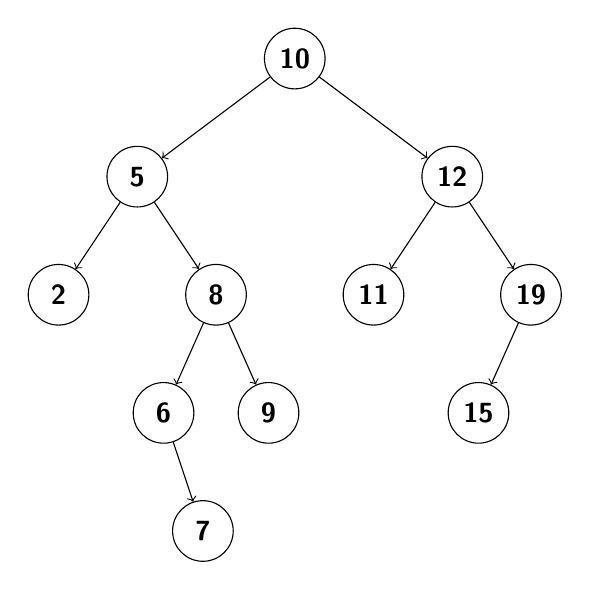
\begin{tikzpicture}[->, level/.style={sibling distance=4cm/#1}] 
                \node [node_num] {10} % ROOT
                child{ node [node_num] {5} 
                    child{ node [node_num] {2}}
                    child{ node [node_num] {8}
                        child{ node [node_num] {6}
                            child[missing]{}
                            child{node [node_num] {7}}
                        }
                        child{node [node_num] {9}}
                    }                     
                }
                child{ node [node_num] {12}
                    child{ node [node_num] {11}}
                    child{ node [node_num] {19}
                        child{ node [node_num] {15}}
                        child[missing]{}
                    }
                }
                ; 
            \end{tikzpicture}
        \end{center}
        \vspace{1cm}
        
        \item Remove: [7, 12, 8, 10]
        
        \begin{center}
            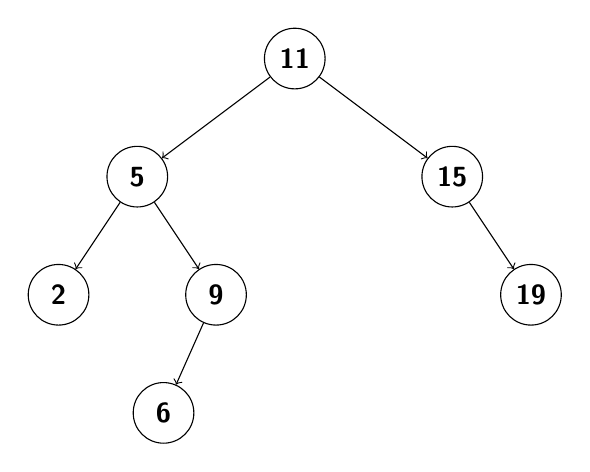
\begin{tikzpicture}[->, level/.style={sibling distance=4cm/#1}] 
                \node [node_num] {11} % ROOT
                child{ node [node_num] {5} 
                    child{ node [node_num] {2}}
                    child{ node [node_num] {9}
                        child{ node [node_num] {6}}
                        child[missing]{}
                    }                     
                }
                child{ node [node_num] {15}
                    child[missing]{}
                    child{ node [node_num] {19}}
                }
                ; 
            \end{tikzpicture}
        \end{center}
    \end{enumerate}
    
    \newpage
    \item Write a function to delete binary trees. Be sure to remove nodes in the proper order, so that none get orphaned.

    \begin{verbatim}
        // Initial call should pass root to clear whole tree.
        void clear(BSTNode* node) {
            if (!node) return;
            
            clear(node->left);
            clear(node->right);
            delete node;
            return;
        }
    \end{verbatim}

    \item Assume nodes in a BST contain 4 data members: {\it data, depth, left, right}.  Write a recursive function that, given a pointer to the root of a BST, will update every node's {\it depth} to it's own depth in the tree.

    \begin{verbatim}
        // Initial call should pass 0 for 'depth'.
        void update_depth(BSTNode* node, int depth) {
            if (node) {
                node->depth = depth;
                update_depth(node->left, depth+1);
                update_depth(node->right, depth+1);
            }
        }
    \end{verbatim}

    \item Briefly explain the difference between in-order, post-order, and pre-order traversals.

    The three terms above signify different methods of traversing a binary tree. From the point of view of the node, in-order signifies visiting the left child, then itself, then the right child; post-order signifies visiting both children before itself; pre-order signifies visiting itself before any children. All three are necessary for different scenarios, as all provide different utility. For example, you cannot delete a node until all children are removed, yet you cannot know the depth of the children without visiting the parent first.

    \item Implement a binary search tree with all of the following methods: constructor, destructor, insert, search, remove.

    \item Let $T$ be a full k-ary tree, where $k=2$ (a.k.a. {\it binary tree}), with $n$ nodes.  Let $h$ denote the height of $T$.
    \begin{enumerate}
        \item What is the minimum number of leaves for $T$?  Justify your answer.

        $$ h + 1 $$
        
        \vspace{0.5cm}
        Example when $h = 0$ : $T$, being a \emph{full tree} can have a minimum of 1 leaf.

        \begin{center}
            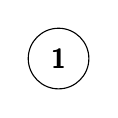
\begin{tikzpicture}[->,>=stealth',level/.style={sibling distance = 4cm/#1,
                level distance = 1.5cm}] 
                \node [node_num] {1} % ROOT
                ; 
            \end{tikzpicture}
        \end{center}
        \newpage

        \item What is the maximum number of leaves for $T$?  Justify your answer.

        $$ 2^h $$
        
        \vspace{0.5cm}
        If we consider the root having height 0, then our maximum number of leaves is when we have a perfect binary tree of height $h$, thus the maximum number of leaves we can have is:
        $$ 1, 2, 4, 8, \ldots, 2^h $$
        \vspace{.5cm}
        
        \item What is the minimum number of internal nodes for $T$?  Justify your answer.

        $$ h $$

        \vspace{0.5cm}
        Considering the smallest tree, with only one node, we can see that it is possible to have 0 internal nodes. 

        \begin{center}
            
\begin{tikzpicture}[->,>=stealth',level/.style={sibling distance = 4cm/#1,
                level distance = 1.5cm}] 
                \node [node_num] {\emph{root}} % ROOT
                ; 
            \end{tikzpicture}
        \end{center}
        \vspace{0.5cm}
        
        \item What is the maximum number of internal nodes for $T$?  Justify your answer.

        $$ 2^h - 1 $$
        
        The maximum number of internal nodes can be expressed as the difference between the number of nodes in a tree, and the number of leaves (since nodes can either be leaves, or be internal). The maximum number of internal nodes occurs when a tree is perfect. The number of nodes in a perfect tree is expressed as $2^{h+1}-1$, the number of leaves in a perfect tree is expressed as $2^h$, therefore:

        $$ (2^{h+1}-1)-2^h = 2^h - 1 $$
    \end{enumerate}

    \item Give a $O(n)$ time algorithm for computing the \verb|height| of the tree, where $n$ is the number of nodes.

    \begin{verbatim}
        // Initial call should pass depth=-1, this special value
        // is returned when the tree is empty.
        int height(BSTNode* node, int h) {
            if (node) {
                return max(
                    depth(node->left, depth+1), 
                    depth(node->right), depth+1)
                )
            } else {
                return depth;
            }
        }
    \end{verbatim}

    \item Show that the maximum number of nodes in a binary tree of height $h$ is $2^{h+1}-1$.

    $$ 1 + 2 + 4 + 8 + \ldots + 2^h = 2^{h+1} - 1 $$

\end{enumerate}

\label{r:lastpage}

\end{document}
    